%! Author = Nhat Huy Vu
%! Date = 9/12/2024

% Preamble

% Document

\subsection*{SIFT features}
Scale-Invariant Feature Transform (SIFT) is a method for detecting and describing local features in images. It transforms image data into scale-invariant
coordinates relative to local features. That means, these features are invariant to scale, rotation, and partially invariant to changes in illumination
and 3D camera viewpoint. These features can be described as aset of vectors~\cite{Lowe.2004}:
\begin{equation}
\{v_1, v_2, ..., v_n\}
\end{equation}
where each $v_i$ is a 128-dimensional vector.\footnote{For further details, see ~\cite{Lowe.2004}.}

The pipeline for calculating SIFT features involves the following steps: %Page 94 of paper Lowe.2004
\begin{enumerate} %Add more concise descriptions for each step later
    \item \textbf{Scale-space Extrema Detection:} This step computes the local extrema of the Difference of Gaussian function convolved with the image, which are
    keypoint candidates. See the next subsection for more details.
    \item \textbf{Keypoint Localization:} The candidate keypoints resulting from the previous step will then go through a refinement process to eliminate
    low-contrast keypoints and poorly localized keypoints along edges, resulting in a set of stable keypoints.
    \item \textbf{Orientation Assignment:} Each keypoint is assigned an orientation based on local image properties.
    \item \textbf{Keypoint Descriptor Generation:} A descriptor is computed for each keypoint using highly distinctive yet as invariant as possible features such
    as local image intensities around the keypoint.
\end{enumerate}

\subsubsection*{Calculation of Scale-Space Extrema}
The first step in calculating SIFT features is to detect stable keypoints across all scales. These are points that are invariant to scale changes. To achieve this, the
image is convolved with a scale-space kernel over a range of scales.

According to Koenderink (1984) and Lindeberg (1994), "the only possible scale-space kernel is the Gaussian function. Therefore, the scale space of
an image is defined as a function $L(x, y, \sigma)$, that is produced from the convolution of a variable-scale Gaussian,
$G(x, y, \sigma)$, with the image $I(x, y)$:

$$
L(x, y, \sigma) = G(x, y, \sigma) * I(x, y)
$$

where * is the convolution operation in x and y, and

$$
G(x, y, \sigma) = \frac{1}{2\pi\sigma^2}e^{-(x^2 + y^2)/2\sigma^2}.
$$"

The convolution operation can be implemented in Python using cv2.GaussianBlur() function (note that this is a discrete approximation of the continuous
Gaussian function). Assume a symmetric kernel size of $3 \times 3$ and a standard deviation of $\sigma$ in both
x and y directions, the function can be called as follows:

\begin{verbatim}
kernel = (3, 3)
sigma = 1.0
cv2.GaussianBlur(src, kernel, sigma)
\end{verbatim}

Stable keypoints in scale space can be detected using scale-space extrema in the Difference of Gaussian function convolved with the image($D(x, y, \sigma)$):

$$
D(x, y, \sigma) = (G(x, y, k\sigma) - G(x, y, \sigma)) * I(x, y) = L(x, y, k\sigma) - L(x, y, \sigma)
$$

To find out the value of $k$, each octave of scale space is divided into s invervals, and the value of $k$ is set to $2^{1/s}$. Then, we must produce
s+3 blurred images for each octave, so that final extrema covers a complete octave. This can be implemented in Python using the following code:

\begin{verbatim}
s = 3
k = 2**(1/s)
octave_images = [cv2.GaussianBlur(src, kernel, sigma * (k**i)) for i in range(s+3)]
\end{verbatim}

The result of this operation is a list of s+3 gaussian images, each with a different scale. Adjacent gaussian images are then subtracted to produce difference-of-gaussian (DoG)
images. After each octave, the image is resized to half of its original size. This can be illustrated in the image below:

\begin{figure}[h]
    \centering
    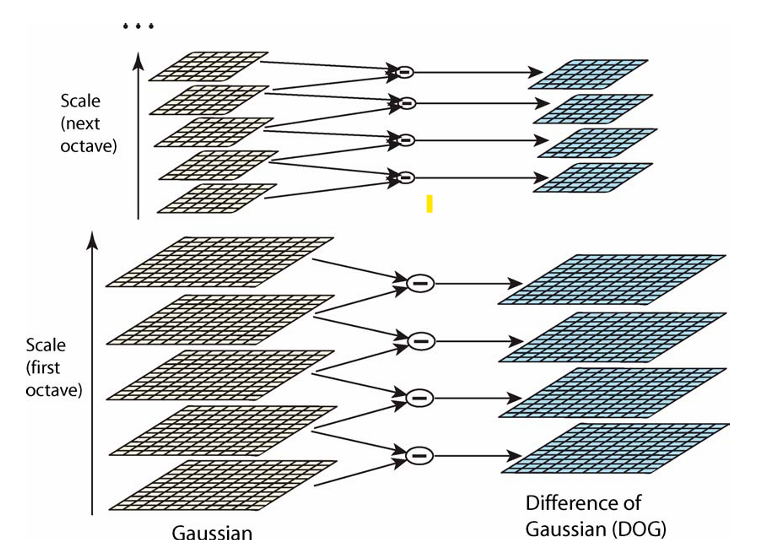
\includegraphics[width=0.5\textwidth]{../images/DoG}
    \caption{Difference of Gaussian images. It can be seen that the image size is reduced by half for each octave~\cite{Lowe.2004}}
    \label{fig:DoG}
\end{figure}

% Add plotted images here later %%%%%

%%%%%%%%%%%%%%%%%%%%%%%%%%%%%%%%%%%%%

For further details, see~\cite{Lowe.2004}.

\subsubsection*{Implementation in Python}
The OpenCV library in Python already provides a function for this operation. Below is an example of how to calculate SIFT features using OpenCV:

\begin{verbatim}
sift = cv2.SIFT_create()
keypoints, descriptors = sift.detectAndCompute(image, None)
\end{verbatim}
